\graphicspath{{02-TOF/Figures/}}


\newcommand{\mchange}[2]{{\color{red}#1}{\color{green}#2}}
\newcommand{\malert}[1]{{\it\color{red}#1}}
\newcommand{\hilite}[1]{{\it\color{blue}#1}}
\newcommand{\Tzero}{\ensuremath{T0}}

\section{Time-of-Flight Detectors}
\label{Sect:TOF}

List of figures
\begin{itemize}
\item PMT charge correlation PMT0 vs PMT1 - maybe, if relevant
\item \hilite{TW calibration of one channel}
\item \hilite{Slab DT before TW correction and after - single pixel.}
\item \hilite{Residual TW}
\item T0 correction for 1 channel - electron peak fit
\item \malert{(?)} Slab DT mean and sigma for all pixels after
  calibration
  \begin{itemize} \it
  \item depends on whether we are comfortable with showing it
  \end{itemize}
\item \hilite{Overall slab DT}
\item Space-point creation efficiency per pixel/slab
  \begin{itemize}\it
  \item this is tricky, the only inefficiency comes from time mismatch
  \item it can point to a fact that some slabs/pixels have something
    wrong with them
  \item it is not measure of performance per se
  \end{itemize}
\item Particle detection efficiency
  \begin{itemize} \it
  \item don't know how to extract from the data, ideally pixel map for
    each TOF
  \end{itemize}

\end{itemize}


\malert{Issues:}
\begin{itemize}
\item should we use word ``counter'' or ``slab''?
\end{itemize}

\subsection{Introduction}
\label{SubSect:TOF_Intro}
% version 01 edited by Maurizio Bonesini 19/2/2018

Three time-of-flight detectors (TOF0, TOF1, TOF2) have been built and
installed at RAL in 2008 and 2009 to measure the position and the time
of crossing particles.  TOF0 and
TOF1~\cite{NOTE145},~\cite{NOTE241},~\cite{2010NIMPA.615...14B} are
placed upstream of the cooling channel, and TOF2~\cite{NOTE286} is
downstream of the channel, mounted in front of the KL, as shown
in~Fig.~\ref{fig:BL}.  The time of flight between two TOF stations
provides particle identification information and can also be used for
momentum measurement. TOF1 served most of the time also as an
experimental trigger.  They have smoothly operated during the
so-called Step~I and
Step~IV~\cite{Rajaram:2015bra},~\cite{2015ehep.confE.521B} running
periods of the MICE experiment and were essential for all the
measurements done.

The good performances of the TOF detectors, over an extended period of time,
has enabled the MICE experiment to characterize fully its muon beams during
Step~I data-taking, by measuring their emittance~\cite{2013arXiv1306.1509T} and
assessing their pion contamination~\cite{2016JInst..11P3001A}.

Each TOF station is made of two planes of fast~1" thick scintillator
counters along X/Y directions (to increase measurement redundancy)
read out at both edges by R4998 Hamamatsu fast photomultiplier
tubes\footnote{one-inch linear focused PMTs with 10 stages, typical
  gain G$\sim$5.7$\times$10$^6$ at -2250~V and B=0~T, rise time
  0.7~ns, transit time spread (TTS)~$\sim$160~ps}.  R4998 PMTs have
been delivered by Hamamatsu in assemblies (H6533MOD) that include the
PMT tube, the voltage divider chain and a 1~mm thick $\mu$-metal
shield, extending 30~mm beyond the photocathode surface.
\mchange{The}{To} increase the count rate stability active dividers
were used, instead of conventional resistive ones.  A simple design
with flat fish-tail PMMA light guides, as \mchange{respect}{opposed}
to tilted ones (to reduce the influence of magnetic field) or Winston
cones, has been chosen to optimize the timing detector resolution
(favouring the collection of straight light) and to allow an easy
mechanical assembly. \malert{any picture or reference here?}  TOF0,
TOF1, and TOF2 have active areas of 40$\times$40~cm$^2$,
42$\times$42~cm$^2$, and 60$\times$60~cm$^2$ respectively.  The slabs
in TOF0 are 4~cm wide, while the slabs of TOF1 and TOF2 are 6~cm wide
respectively.  The PMT\mchange{s}{} signal, after $\sim$34~m long
RG213 cable and a $50\%-50\%$ passive splitter, arrive to a
leading-edge CAMAC Lecroy 4115 discriminator followed by a CAEN V1290
TDC for time measurements and to a CAEN V1724 FADC for pulse-height
measurements, to correct time-walk. As reported in
reference~\cite{NOTE241}, RG213 cables\footnote{CERN type C-50-6-1,
  with rated delay 4.08 ns/m} have a better temperature stability than
conventional RG58 cables. Their delay have been individually measured
in laboratory, before installation in the experimental hall.  Time
calibration of individual counters has been done with impinging beam
particles by using the detector X/Y
redundancy~\cite{NOTE251}. \malert{This is too vague. Calibration will
  be covered later. What does counter refer to here?}

Due to the low residual magnetic field produced by the last quadrupole
of the beam line in the proximity of the TOF0 detector ($\leq$50~G),
the used conventional PMTs had to use elongated $\mu$-metal shielding.
The other two TOF stations (TOF1/TOF2) had to work instead in the
stray fields of the cooling channel solenoids, that are only partially
shielded by a 100~mm thick annular iron plates. As residual magnetic
fields are up to 0.13~T (with a component along the PMTs axis up to
0.04~T), a local or global magnetic shielding for TOF1 and TOF2
detectors had to be envisaged.  The local shielding option was chosen,
at the end, for convenience and easiness of implementation.  As
magnetic shielding is a mass effect, box-shaped soft iron shielding
are more effective than cylindrical ones. This idea pioneered in the
D0 experiment has been tested in the case of MICE using different
geometrical configuration for the iron shielding boxes and different
iron materials (e.g. Fe360, ARMCO\footnote{ARMCO steel from AkSteel is
  a pure iron with a maximal carbon content of $0.025\%$ and very high
  magnetic saturation},~etc).  The problem is usually the longitudinal
component of the magnetic field, while the orthogonal component may be
more easily shielded.  Systematic studies have been done, using a
built on purpose solenoid of 23~cm inner diameter, 40~cm
length\footnote{built by TBM srl, Uboldo (VA), Italy} and are fully
reported in reference~\cite{2012NIMPA.693..130B}.  A composite
structure based on the 1~mm $\mu$-metal shielding of the H6533Mod
assemblies and an external additional 6$\times$6~cm$^2$
(5.6$\times$5.6~cm$^2$) ARMCO box, 15~cm long, with an internal hole
of 3.2~cm diameter has been adopted for the PMT's magnetic shielding
of TOF2 (TOF1)~\cite{NOTE455}.  Fig.~\ref{fig:TOF1} show how the local
shielding has been implemented in TOF2, using different sheets of
ARMCO to make a ``single bar structure'' for all the PMTs of one side,
instead of single boxes for individual PMTs. The effective shielding
amounts to $\sim$6.6~cm of ARMCO thickness, with extra shielding
effect due to the fact that all bars shielding the TOF2 PMTs are
magnetically linked between them and to both the KL shielding and the
shielding plate making a single magnetic loop.
\begin{figure}
  \begin{center}
  \includegraphics[width=9cm,angle=-90]{./02-TOF/Figures/TOF2.eps} \\
  \caption{Exploded view of the TOF2 detector magnetic shielding for one row of PMTs.}
  \label{fig:TOF1}
  \end{center}
\end{figure}
Fig.~\ref{fig:TOF2} shows some steps of the assembly procedure for the TOF2
detector at INFN MIB mechanics workshop.
\begin{figure}
  \begin{center}
  \includegraphics[width=0.24\columnwidth]{./02-TOF/Figures/TOF_assembly_a.png}
  \includegraphics[width=0.24\columnwidth]{./02-TOF/Figures/TOF_assembly_b.png}
  \includegraphics[width=0.24\columnwidth]{./02-TOF/Figures/TOF_assembly_c.png}
  \includegraphics[width=0.24\columnwidth]{./02-TOF/Figures/TOF_assembly_d.png}
  \caption{Assembly of TOF2 at INFN MIB mechanics workshop. Left to right: from the bare magnetic shielding to the installed counters of a plane.}
  \label{fig:TOF2}
  \end{center}
\end{figure}

\malert{The paragraph above is rather detailed, with many things that
  could be explained incorrectly. Should be made brief, unless full
  technical design description is required.}


\malert{The following paragraph is summarising the performance. It
  states overly optimistic performance.}

\malert{reformulate ---} For what attains performances\malert{---},
TOF0, TOF1, and TOF2 had timing resolutions around 50-60 ps
respectively \malert{(currently observed $\sim$110~ps)}, over the 8
years running period, consistent with design requirements, with the
spatial resolution around 1~cm. \malert{We don't use any special
  reconstruction method. Resolution kept at 4 cm or 6 cm for TOF0 or
  TOF1 and TOF2 respectively. Do we say resolution = 1/2 of strip
  width or $1/\sqrt{12}$?}  Fig.~\ref{fig:TOF3}~shows distributions of
the time of flight between TOF0 and TOF1 where electrons, muons and
pions fall into three well defined peaks.
\begin{figure}
  \begin{center}
    \includegraphics[width=0.6\columnwidth]{./02-TOF/Figures/TOF.png}
    \caption{Time of flight between TOF0 and TOF1 for a ``pion''
      beam. From the left: the well separated electron, muon and pion
      peaks.}
    \label{fig:TOF3}
  \end{center}
\end{figure}


\malert{What is currently the main purpose of TOFs? This determines
  the requirements on the performance. Will need to tell that current
  T-o-F measurement has sufficient resolution, which appears to be
  $\sim$100-120~ps}


Error of the time-of-flight measurement is a combination of intrinsic
resolution of each TOF station and errors in the calibrations of
individual \malert{scintillation counters}. The total error of t-o-f
as measured by stations $i$ and $j$ is considered as:
%
\begin{equation}
  \label{eq:tof:err}
  \sigma_{\text{TOF}_{ij}} = \sqrt{ \sigma^2_{i} + \sigma^2_{j} +
    \sigma^2_{\text{calib}} } .
\end{equation}

Individual uncertainties $\sigma_i$ are assumed to be statistically
uncorrelated. Error of the calibration method, $\sigma_\text{calib}$,
consists of uncertainties correlated and uncorrelated between the
stations.


\subsection{TEMPORARY - Plots}

\begin{figure}
  \begin{center}
  \includegraphics[clip,trim=0 8.5cm 10cm 0, width=9cm]{01_tw_example} \\
  \caption{}
  \label{fig:TW}
  \end{center}
\end{figure}

\begin{figure}
  \begin{center}
  \includegraphics[clip,trim=0 0 10cm 8.5cm, width=9cm]{02_slab_dt_resolution_tw_effect} \\
  \caption{}
  \label{fig:SlabDTTW}
  \end{center}
\end{figure}

\begin{figure}
  \begin{center}
  \includegraphics[width=9cm]{03_residual_tw_example} \\
  \caption{}
  \label{fig:ResTW}
  \end{center}
\end{figure}



\begin{figure}
  \begin{center}
  \includegraphics[clip,trim=0 0cm 10cm 0, width=9cm]{04_tof_t0_example} \\
  \caption{}
  \label{fig:tofT0}
  \end{center}
\end{figure}


\begin{figure}
  \begin{center}
  \includegraphics[width=15cm]{05_slab_dt_offset_by_pixel_2d} \\
  \caption{}
  \label{fig:SlabDToffsetByPixel}
  \end{center}
\end{figure}


\begin{figure}
  \begin{center}
  \includegraphics[width=15cm]{06_slab_dt_resolution_by_pixel_2d} \\
  \caption{}
  \label{fig:SlabDTresByPixel}
  \end{center}
\end{figure}



\begin{figure}
  \begin{center}
  \includegraphics[width=15cm]{07_overall_slab_dt} \\
  \caption{}
  \label{fig:SlabDtAll}
  \end{center}
\end{figure}


\begin{figure}
  \begin{center}
  \includegraphics[width=15cm]{08_sp_eff_by_pixel_2d} \\
  \caption{}
  \label{fig:SpEffByPixel}
  \end{center}
\end{figure}




\subsection{Calibration Method}
\begin{itemize}
\item Describe the method. Based on MICE note 251.

\item \malert{TOF NIMA paper says that measured time resolution of the
    CAEN TDC was 22~ps/count, as opposed to declared 25~ps!}

\item  Some description of the calibration method is also described in the
  paper.


\item  \malert{There's a short description of the method also in Rayner's
    Thesis, Section 3.2.1 and Appendix B (this is improved method to
    extract more calibration constants for proper x,y measurements,
    Rayner claims $\sim$1~cm resolution; our current resolution = slab
    width / sqrt(12) $\sim 1.2 - 1.7$ ).}

\end{itemize}

Measurement of time traversal of a particle through a TOF station is
influenced by several factors at the hardware level. When a particle
crosses the plastic scintillator, there is a short delay in light
production. There are often at least two components to the light: the
first one is fast with a characteristic scintillation time of
$\sim$1~ns, and second being much slower with characteristic time
$\sim$10~ns \malert{(double check the times)}. Contribution of each
component changes with the ionisation density and hence with particle
type.

After generation, scintillation light propagates to the ends of each
scintillator slab where it is detected by photomultiplier tubes. The
light-travel time depends on the distance of the particle crossing
from the PMT. The length of slabs in TOF0, TOF1, and TOF2 are 40~cm,
42~cm, and 60~cm, respectively. This translates to about 3~ns, 3.1~ns,
and 4.4~ns, respectively, as the effective light propagation speed in
the scintillator was found to be approximately 13.5~cm/ns.

Next delays are introduced by the transit times of each PMT and the
cable that lead the signal to the electronics. These times are
specific for each individual PMT channel and needs to be determined
in dedicated measurements.

The times of each signal of a PMT are measured as times of signal threshold
crossings in a simple linear discriminator. This introduces bias in
the measured time dependent on the total charge of the signal, effect
referred to as time-walk.

Signal times of each channel are recorded in TDC boards. Readout of
the whole system is triggered by having a signal in TOF1 station. Time of
the channel that caused the readout is also recorded in each TDC board
and is used as a reference time. Depending on where the particle
crosses through TOF1 station, this trigger time will be issued by
different PMTs, and consequently the reference time will have a bias
dependent on the position of TOF1 crossing.

The final time measurement in each station determined as an average of
the times of individual channels. This way, different distance from
the point of crossing to each side of the scintillator slabs does not
matter anymore, because the average of the times of the 2 PMTs does
not depend on it.

Corrections which need to be made to the measured times are then the
time-walk correction, PMT channel specific delay time $T0$, and
correction for reference trigger time delay.


\subsubsection{Time-walk Correction}
\begin{itemize}
\item \malert{Fig of a selected PMT TW 2D hist. + Profile + Fit}
\item  \malert{Fig of residual TW.}
\item  \malert{Fig of Slab DT before TW
    correction and after.}
\end{itemize}
Time walk was considered to be constant property of each channel. The
same correction was used for all runs.

First correction to the measured time of each channel is time-walk
correction. The correction was determined by looking time difference
between two selected channels from two crossing slabs.

Correction was first determined for reference slabs, middle slabs in
each plane. Pixel corresponding to their crossing was always well
populated with particles crossing it which provided large statistics
to limit the charge in one of the slabs to a small region around its
maximum and to use it as reference time which was little affected by
the time walk. Time walk of PMTs in the other slab could easily by
determined from the measured time with respect to the limited
reference channel.

After provisional determination of time-walk of the reference slabs,
time-walk of all the PMT channels was determined by looking at events
in pixels corresponding to the crossing with the reference slab.

A time-walk correction curve was fitted to the data. First, a profile
was created and then function
%
\begin{equation}
  \newcommand{\ADC}{\text{ADC}}
  \label{eq:twf}
  f(\ADC) = P_1 + \frac{P_2}{\ADC - P_0} + \frac{P_3}{\left(\ADC - P_0\right)^2}.
\end{equation}
%
Where possible, parameter $P_3$ was fixed to 0. For some PMTs such fit
would not follow the measured trend and the additional parameter was
added to the fit.


Example of time-walk in a reference channel after the first round of
reference calibrations is in Figure~X. Example of time walk of a
channel with respect to pre-corrected time in a reference slab is
shown in Figure~Y.

Figure~Z shows distributions of time differences between horizontal
slab 4 and vertical slab 5 before and after time walk correction. The
width of the distribution is significantly decreased. The mean of the
distribution is not centered at 0 as differences in delays \Tzero{} due to
individual PMTs and their cables were not accounted for, yet.

\subsubsection{Trigger Delay Correction}
\newcommand{\Tdelay}[2]{\ensuremath{T_{\text{tr}}^{#1,#2}}}

Station TOF1 was used to trigger readout of the whole system. Time of
it's trigger signal was used as a reference signal to which times of
each channel of all 3 stations were measured. Two-fold coincidence of signals
crossing threshold in PMTs on both sides of a slab is required.
%
For an incoming particle the trigger signal is given by the first of
the twofold coincidences from slab i and slab k. The time of the
coincidence signal is the time of the latest signal arriving to the
logic unit.
%
Which PMT channel will be causing trigger depends on the position
within the slab of the particle crossing and the \Tzero{} delays of
individual PMTs. Assuming that light arrival time does not change
significantly across a pixel and no other effects influence signal
arrival one can expect that passage of a particle through a given
pixel causes always the same time sequence of PMT signals and the
delay of the trigger signal will be that of one particular channel in
each pixel. This assumption, however, does not hold for all
pixels. The main reason being the time walk effect which biases each
channel differently and in some pixels results in more than 1 PMT
channel generating the trigger signal.

The trigger signal delay of each pixel was measured relative to the
central pixel of TOF1 station. Times of each PMT were corrected for
time walk first. Mean times of PMTs in reference slabs, horizontal
slab 3 and vertical slab 3, were compared for each pixel.

\newcommand{\TW}{\ensuremath{\text{TW}}}
\newcommand{\PMT}{\ensuremath{\text{PMT}}}
${t_\TW}_{i,j}^\PMT$

{
\newcommand{\ttrig}[3]{\ensuremath{{t_\TW}_{#2,#3}^{#1}}}
\newcommand{\mean}[1]{\ensuremath{\left< #1 \right>}}
\begin{align}
  %\label{eq:trigdel}
  &\frac12\sum_{\PMT}
    \mean{\ttrig{\PMT}{3}{j}} -
    \mean{\ttrig{\PMT}{3}{3}} \label{eq:trigdel:horiz} \\
  &\frac12\sum_{\PMT}
    \mean{\ttrig{\PMT}{i}{3}} -
    \mean{\ttrig{\PMT}{3}{3}} \label{eq:trigdel:vert} \\
  &\frac14\sum_{\PMT}
    \left(
    \mean{\ttrig{\PMT}{i}{j}} - \mean{\ttrig{\PMT}{i}{3}} +
    \mean{\ttrig{\PMT}{i}{j}} - \mean{\ttrig{\PMT}{i}{3}}
    \right) \label{eq:trigdel:both}
\end{align}
}

For pixels not defined by the reference slabs, we can compare
estimated delay times \Tdelay{i\neq3}{j\neq3} arrived to from the
vertical and horizontal reference slab, 1st and 2nd part of Equation
(\ref{eq:trigdel:both}), respectively.

Figure~X shows comparison of time-walk corrected recorded times in a
channel for particles passing through different pixels. The variation
in position of the peaked distributions is clearly visible.

Figure~Y shows times measured in a channel in TOF0 station for
particles crossing the station's central pixel (4,5). Times
before correction for the trigger signal delay are compared to times
after the correction.

\subsubsection{$T0$ Correction}

Times in each channel were corrected for the channel specific delays
caused by each PMT and by cable lengths. The correction was extracted
from channel times corrected for time walk and trigger signal
delay. After that, TOF1 stations' times differ only by the channel
specific delays. Constant offests were applied such that time distributions
in TOF1 were centered at 0.

Times in TOF0 and TOF2 stations reflected the time of flight of
individual particles to and from TOF1 and the channel delays
\Tzero. Distribution of the times in those station show 3-peaked
structure, where the most isolated peak at lowest tome-of-flight
corresponds to electrons in the beam which travel at speed of
light. Their time of flight was calculated from distances from TOF1
station, 8.XX~m and 8.xx~m for TOF0 and TOF1, respectively. Figure~Y
shows position of the electron peak in one channel of TOF0 before and
after the last correction. Right hand side of the figure compares
time distribution of all channels before and after the correction.

Due to the presence of focusing fields in the beam-line section
between TOF0 and TOF1 stations, particles did not travel in a straight
line in that section. Deviation from a straight line was dependent on
the initial direction and momentum of the particles entering the
section. The effect was estimated \malert{\cite{RAYNER}} in
simulations to be of an order of $\sim$30~ps. This effect caused a
small bias in the calibrations.



\subsection{Reconstruction}

\begin{itemize}
\item slab hits - must have PMT over threshold on both sides
\item only first recorded hits in the readout (per trigger) are considered
\item times corrected for TW, TrigT and T0
\item corrected slab time is the average of corrected times of each PMT
\item ``Space Point'' (SP) is created for each combination of 2 cross
  slabs where the corrected slab times fall within \malert{3 ns}.
\item coordinate of the SP is placed in the middle of the station
  along the beam axis (where the two slab planes touch each other) and
  in the center of the slabs in the transverse direction.
\item the time of the SP is the average of the slab times of the slabs
  it was reconstructed from.
\end{itemize}

Recorded signals in all PMT channels are processed in the following
way. First, signals in opposite PMTs of a slab are paired. Recorded
times are corrected for time walk, channel delay \Tzero{}, and for the
delay of the trigger signal. This requires that the trigger pixel in
TOF1 station is determined.

Pixel area where the particle crossed the station is searched by
attempting to match all possible combinations of slab signals in each
plane. Transverse slabs are matched if their corrected times fall
within a 4-ns window. A space point is then created with spatial
coordinates centered at centre of the pixel in the transversal
direction and middle of the station in the longitudinal
direction. Time of the space point is calculated as an average of the
times of each slab.


\subsection{Performance}
\label{SubSect:TOF_Performance}

\malert{Several figures are already in the TOF NIMA paper.}

Figures to show here:
\begin{itemize}
\item Slab DT - selected slabs/counters + overall TOFs
\item ToF10 - + detail of electron peak
  \begin{itemize} \it
  \item will need to argue why the peak is broader than stated
    resolution
  \item the effect of electron's flight path due to focusing fields is
    non-negligible - use estimates from Rayner's thesis
  \end{itemize}
\item Space-point reconstruction efficiency
  \begin{itemize}
  \item shows that slab hits are within the required cut
    \begin{itemize}
    \item events with 2 slab hits only
    \end{itemize}
  \item inefficiency from:
    \begin{itemize}
    \item only single slab hit by different particles in the given
      spill/bunch
    \item this may be due to inefficiency of hit creation when
      particle crosses by the edge of the slab -- see Rayner's
      thesis/presentations
    \item two particles share one slab - earlier particle's hit only
      considered - but this is not considered in these plots (only 2
      slab hits recorded)
    \end{itemize}
  \end{itemize}
\item Stability of electron peak - run by run position of electron peak!
\item particle detection efficiency - how to show?
\item Resolution
  \begin{itemize}
  \item Slab DT for all TOFs, show similar performance, although
    they have different construction.
  \end{itemize}
\item \malert{(?)}Efficiency
\end{itemize}


\subsubsection{Low-level Characterisation}

\malert{maybe leave this out, likely not necessary}

\begin{itemize}
\item PMT charge correlation PMT0 vs PMT1 - maybe, if relevant
\item Residual TW - this should go to the calibration section
\item Slab DT
\end{itemize}





% \subsubsection{Time-of-Flight Resolution and Efficiency}

% \begin{itemize}
% \end{itemize}


%%% Local Variables:
%%% mode: latex
%%% TeX-master: "../Systems-performance"
%%% End:
